\subsection{Результат выполненной работы}

В процессе работы над платой были выполнены вышеописанные этапы. На основе принципиальных схем, разработанных в разделе "Схема устройства", был создан проект печатной платы\cite{altium_docs}.
\begin{figure}[ht]
    \centering
    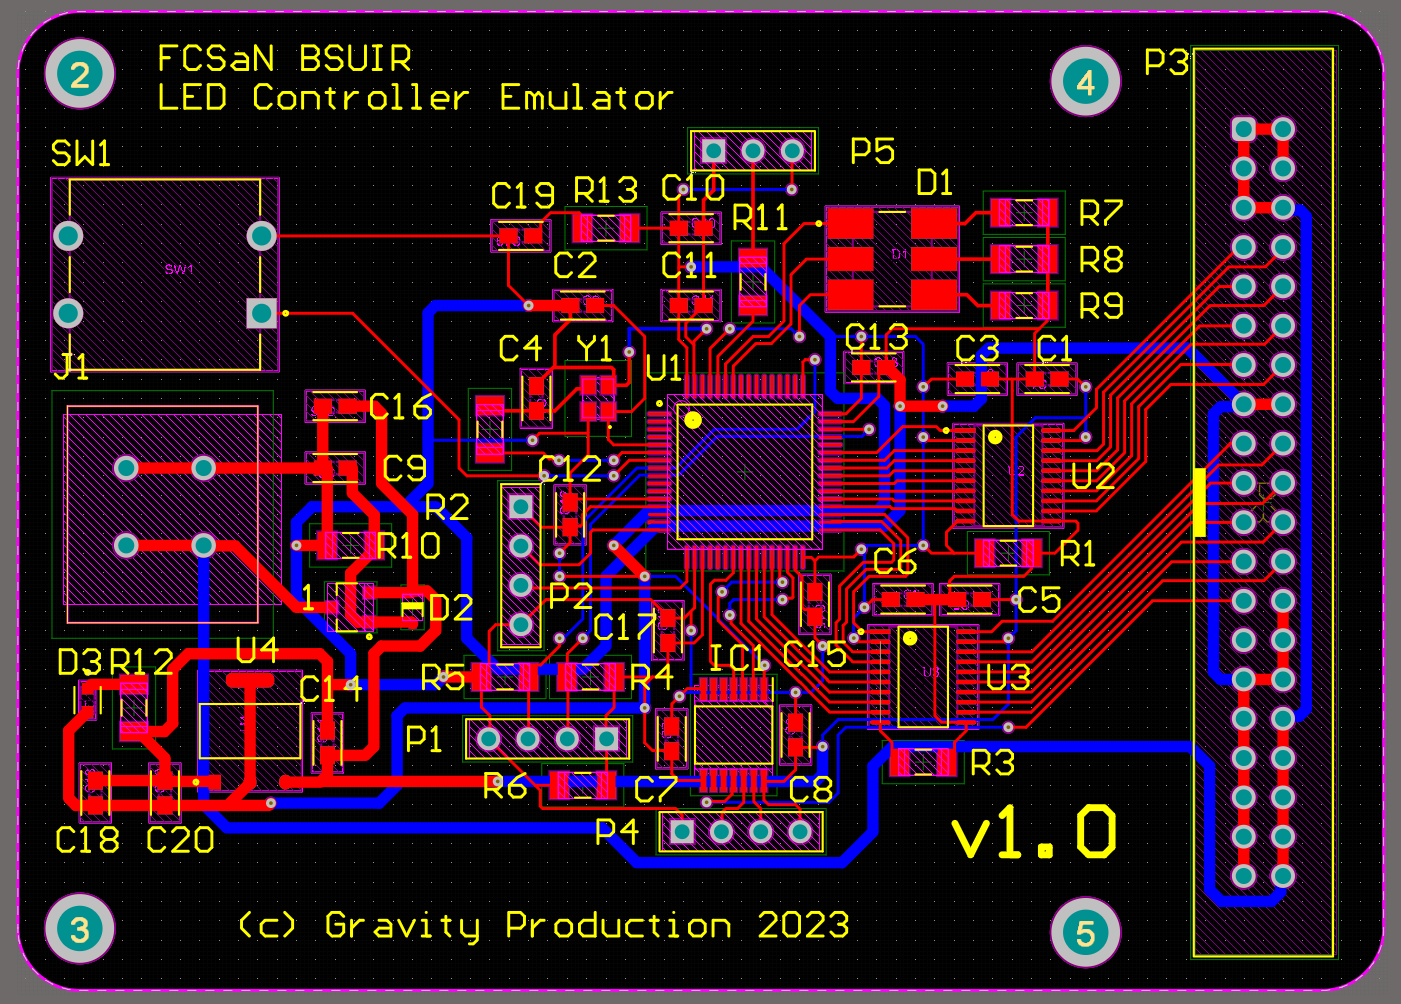
\includegraphics[width=0.65\linewidth]{\commonSecPathPrefix/sec_7/content/pcb.png}
    \caption{Спроектированная печатная плата}
\end{figure}
Для более наглядного представления печатной платы был создан 3D - рендер, который представлен на рисунке ниже.
\begin{figure}[ht]
    \centering
    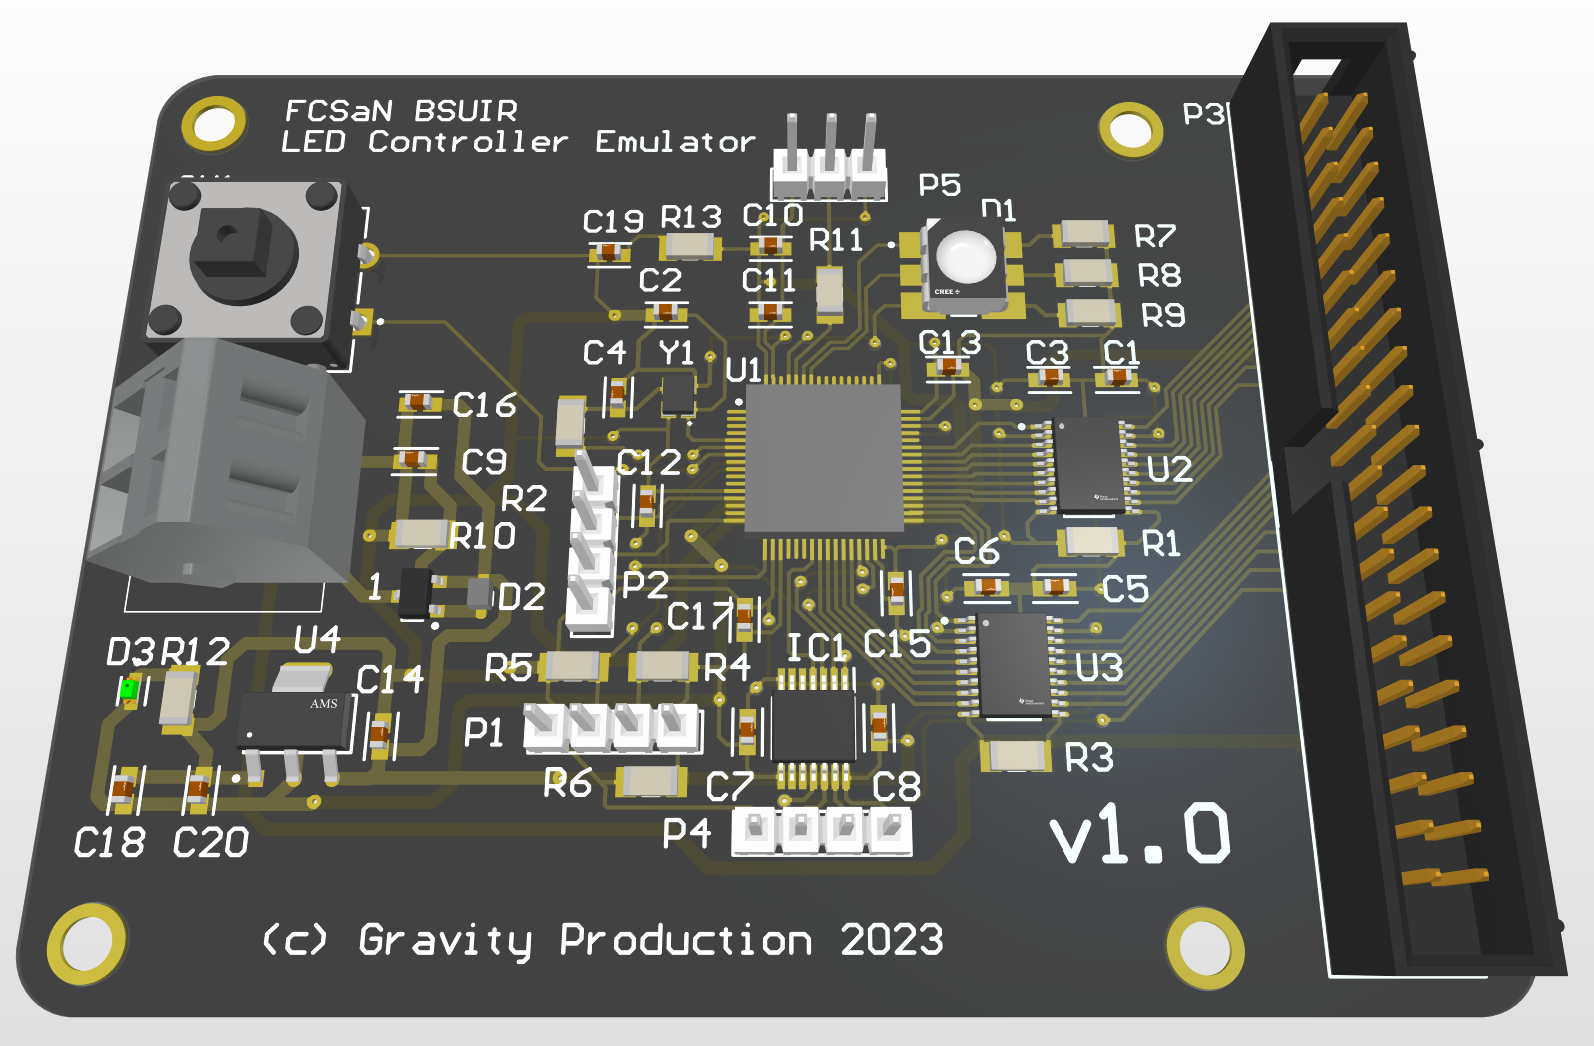
\includegraphics[width=0.65\linewidth]{\commonSecPathPrefix/sec_7/content/3d.png}
    \caption{3D - рендер спроектированной платы}
\end{figure}
Рендер показывает основные элементы платы, а также ее расположение в корпусе устройства.


Компоненты расположены на плате таким образом, чтобы обеспечить эффективное охлаждение и удобство сборки. Крепежные элементы расположены по углам платы и обеспечивают надежное ее крепление к корпусу устройства.


Рендер позволяет оценить внешний вид платы и убедиться в правильности ее размещения в корпусе устройства.